\documentclass[]{beamer}
\usepackage[utf8]{inputenc}
\usepackage{xeCJK}
\usepackage{graphicx}
\usepackage{subfigure}
\usepackage{mathtools}
\usepackage{utopia} %font utopia imported
\usetheme{CambridgeUS}
\usecolortheme{dolphin}
\usefonttheme{professionalfonts}
\usepackage{natbib}
\usepackage{hyperref}
\usepackage{fontspec}
\usepackage{setspace}
\usepackage{float}
% \usepackage{enumitem}

\setCJKmainfont{SourceHanSansSC-Regular.otf}[Path=../, BoldFont=bold.otf]

\setbeamerfont{title}{size=\Large}
\setbeamerfont{subtitle}{size=\small}
\setbeamerfont{date}{size=\small}
\setbeamerfont{institute}{size=\small}

\setstretch{1.3}
% \setlength{\parindent}{2em}
% \setlength{\parskip}{0pt}

% \setlist[itemize]{leftmargin=2em}

% ↓↓↓ Modify this ↓↓↓
\title{高等数学I\quad 习题课04}
\subtitle{数列的极限}
\date[2025.10.9]{2025.10.9}
% ↑↑↑ Modify this ↑↑↑

\author[上海科技大学]{}
\institute[]{上海科技大学}



\begin{document}

\begin{frame}
    \vspace{15pt}
    \titlepage
\end{frame}

% \begin{frame}{Quiz}
%     \[
%     \text{\Huge 18:00 - 18:20}
%     \]
% \end{frame}

\begin{frame}{目录}
    \tableofcontents
\end{frame}

\AtBeginSection[ ]
{
\begin{frame}{目录}
    \tableofcontents[currentsection]
\end{frame}
}

% ↓↓↓ Modify From This ↓↓↓

\section{杂项}

\begin{frame}{及时总结}
    \begin{itemize}
        \item 数学学习类似于一场魂类游戏
        \item 每一个版块,都有自己的难点,一个需要攻克的Boss
        \begin{itemize}
            \item 在不断的尝试与失败中积累经验
            \item 对过去的经验加以总结,重新出发
        \end{itemize}
        \item 每一个板块结束后,找到自己的“赐福”,总结所学到的知识,进行“存档”
        \item 注意\textbf{难度曲线}
    \end{itemize}
\end{frame}

\begin{frame}{难度曲线}
    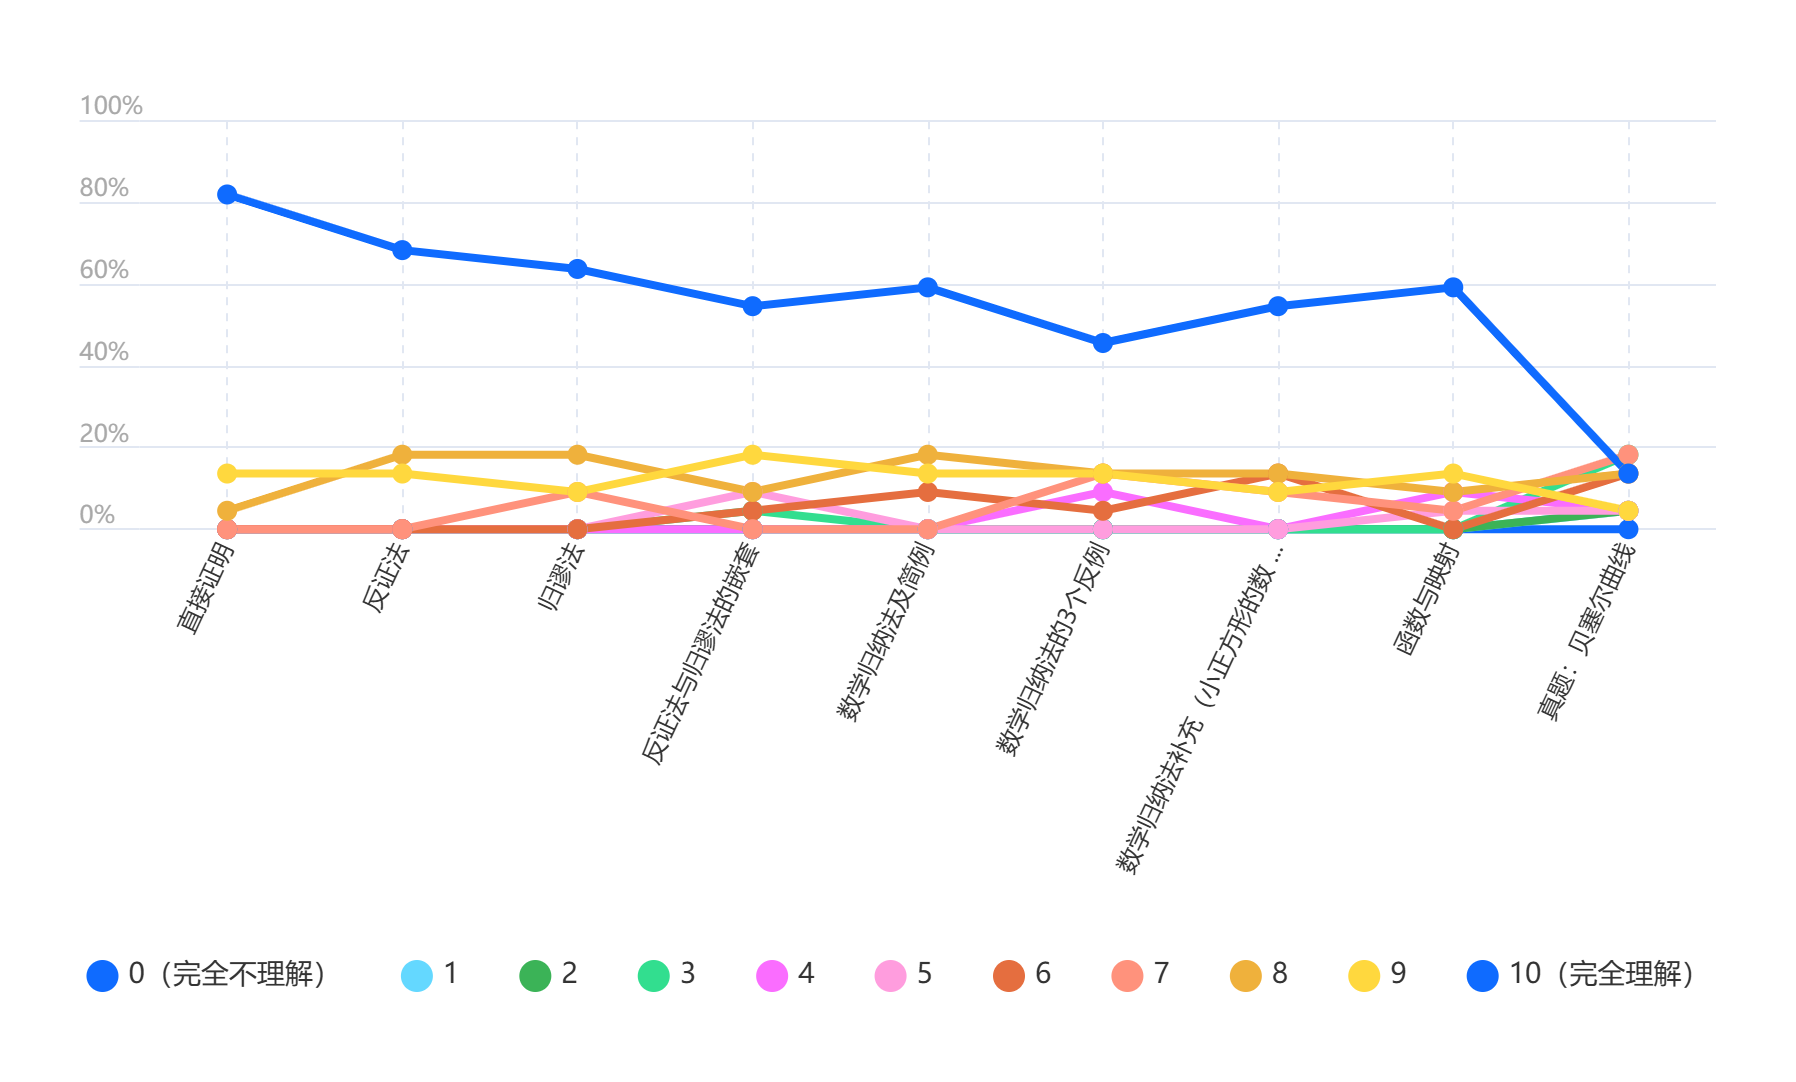
\includegraphics[width=\linewidth]{chart (1).png}
\end{frame}

\begin{frame}{难度曲线}
    \begin{itemize}
        \item 游戏:先难后易
        \begin{itemize}
            \item 难点通过后,只要再一点就能成功
        \end{itemize}
        \item 课业:先易后难
        \begin{itemize}
            \item 从简单的小知识点积累经验与信心
            \item 从大量的小板块中提炼核心以应对大的难点
        \end{itemize}
    \end{itemize}
\end{frame}

\begin{frame}{关于习题课02 反馈}
    \begin{columns}
        % 左栏:文字
        \begin{column}{0.5\textwidth}
            \begin{figure}[H]
                \centering
                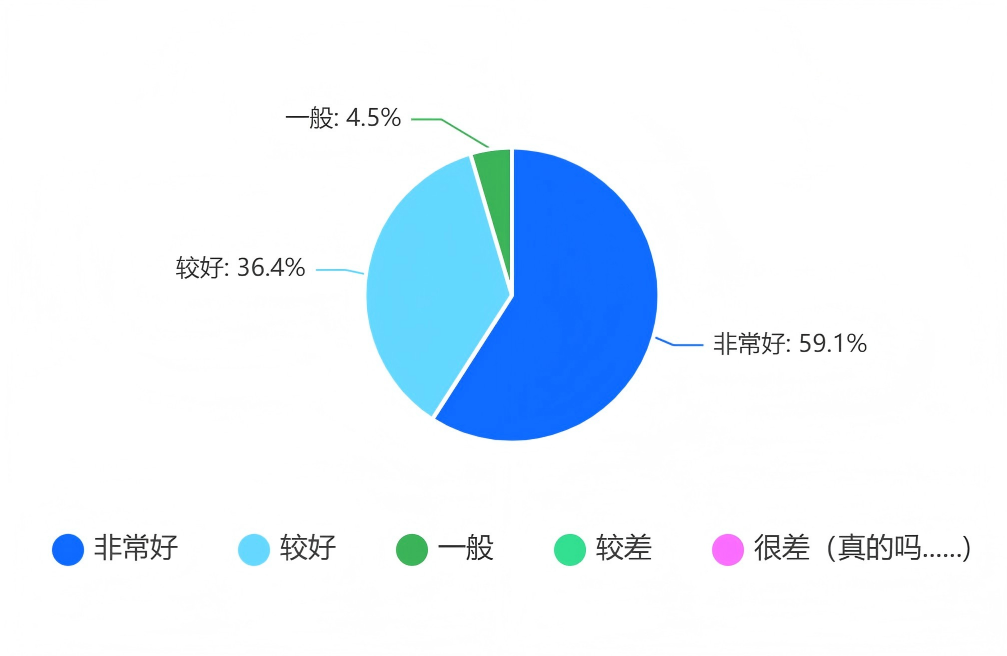
\includegraphics[width=1.0\linewidth]{quality.png}
                \caption{课程质量}
            \end{figure}
        \end{column}

        \begin{column}{0.5\textwidth}
            \begin{figure}[H]
                \centering
                
\includegraphics[width=1.0\linewidth]{atmosphere.png}
                \caption{课堂氛围}
            \end{figure}
        \end{column}
    \end{columns}
\end{frame}

\begin{frame}{关于习题课02 反馈}
    \begin{itemize}
        \item PPT空白多留一些方便记笔记
        \begin{itemize}
            \item 可以使用笔记软件内的增加页面功能
        \end{itemize}
        \item 覆盖面再广一些
        \begin{itemize}
            \item 各人教学风格各有不同,个人倾向于增加内容深度而非广度
        \end{itemize}
    \end{itemize}
\end{frame}

\begin{frame}{贝塞尔曲线}
    贝塞尔曲线是设计与工程上常用的参数曲线.

    平面上一条$n$次贝塞尔曲线由$n+1$个互不相同的控制点
    \[
    P_0(x_0,y_0), P_1(x_1,y_1), \cdots ,P_n(x_n,y_n)
    \]
    决定.其参数方程$B_{P_0P_1\cdots P_n}(t)$可以用下面的递推式表达:
    \[
    B_{P_0}(t)=P_0
    \]\[
    B_{P_0P_1\cdots P_n}(t)=(1-t)B_{P_0P_1\cdots P_{n-1}}(t)+tB_{P_1\cdots P_n}(t),\ 0\le t\le 1.
    \]
\end{frame}

\begin{frame}{贝塞尔曲线}
    \begin{enumerate}
        \item[(1)] 写出一条一次贝塞尔曲线的参数方程,并用文字准确地描述这条曲线.
        \item[(2)] 计算一条二次贝塞尔曲线对参数$t$的二阶导函数(用其三个控制点的坐标表示).
        \item[(3)] 对三个不共线的控制点$P_0,P_1,P_2$,论证二次贝塞尔曲线是一条抛物线(提示:可将上一问的结果与某物理场景对比).
        \item[(4)] 证明
        \[
        B_{P_0P_1\cdots P_n}(t)=\sum_{i=0}^{n}{n\choose i}(1-t)^{n-i} t^i P_i.
        \]
    \end{enumerate}
\end{frame}

\section{数列的极限}
\subsection{定义}
\begin{frame}{定义}
    对数列$\{x_n\}$,若存在数$A$,$\forall \epsilon>0,\exists N\in \mathbb{N}$,使得当$n>N$时,
    \[
    |x_n-A|<\epsilon
    \]
    则称数列$\{x_n\}$的\textbf{极限}为$A$,或称数列$\{x_n\}$\textbf{收敛},且收敛于$A$,记为
    \[
    \lim_{n\rightarrow\infty}x_n=A \text{ 或者 }\ x_n\rightarrow A\quad (n\rightarrow\infty)
    \]
    \color{red}?
\end{frame}

\begin{frame}{定义}
    对数列$\{x_n\}$,若存在数$A$,$\forall \epsilon>0,\exists N\in \mathbb{N}$,使得当$n>N$时,
    \[
    |x_n-A|<\epsilon
    \]
    则称数列$\{x_n\}$的\textbf{极限}为$A$,或称数列$\{x_n\}$\textbf{收敛},且收敛于$A$,记为
    \[
    \lim_{n\rightarrow\infty}x_n=A \text{ 或者 }\ x_n\rightarrow A\quad (n\rightarrow\infty)
    \]
    数列极限的定义,究竟在描述什么?
\end{frame}

\begin{frame}{Game}
    Alice 和 Bob 在玩一个与数列有关的游戏.给定数列$\{a_n\}$,实数$L$
    \begin{enumerate}
        \item Alice 选定一个正数$\epsilon$
        \item Bob 选定一个自然数$N$
        \item Alice 选定一个大于$N$的自然数$n$.
    \end{enumerate}
    如果$|a_n-L|<\epsilon$,则Bob赢,否则Alice赢.
    \begin{itemize}
        \item 思考:双方会为了赢采取什么策略?
    \end{itemize}
\end{frame}

\begin{frame}{Game - Strategy}
    \begin{itemize}
        \item Alice
        \begin{itemize}
            \item 希望 $|a_n-L|\ge\epsilon$. 因此,$\epsilon$越小越有利于Alice取胜.
        \end{itemize}
        \item Bob
        \begin{itemize}
            \item 希望 $|a_n-L|<\epsilon$. 选择越大的$N$越能限制Alice选择$n$的范围,进而防止Alice选出使得$|a_n-L|<\epsilon$不成立的$n$.
            \item 因此,$N$越大越有利于Bob获胜.
        \end{itemize}
    \end{itemize}
\end{frame}

\begin{frame}{Game - 必胜策略}
    \begin{itemize}
        \item 分别在什么条件下,Alice和Bob各有必胜策略?
        \item 对于Bob\dots
        \begin{itemize}
            \item 对于\textbf{任意}的$\epsilon>0$,总能找到一个自然数$N$,使得对于所有的$n>N$,$|a_n-L|<\epsilon$都成立.
            \item $\forall \epsilon >0,\ \exists N\in \mathbb{N},\ s.t.\ \forall n>N,\ |a_n-L|<\epsilon.\quad \Leftrightarrow\quad \lim\limits_{n\rightarrow\infty}a_n=L$
        \end{itemize}
        \item 对于Alice\dots
        \begin{itemize}
            \item 对于\textbf{任意}的$N$, 总能找到一个实数$\epsilon >0$,使得存在一个$n>N$,$|a_n-L|\ge\epsilon$成立.
            \item $\forall N\in\mathbb{N},\ \exists \epsilon>0,\ s.t.\ \exists n>N,\ |a_n-L|\ge\epsilon.$
            \item \color{red}?
        \end{itemize}
    \end{itemize}
\end{frame}

\begin{frame}{Game - 必胜策略}
    \begin{itemize}
        \item 分别在什么条件下,Alice和Bob各有必胜策略?
        \item 对于Bob\dots
        \begin{itemize}
            \item 对于\textbf{任意}的$\epsilon>0$,总能找到一个自然数$N$,使得对于所有的$n>N$,$|a_n-L|<\epsilon$都成立.
            \item $\forall \epsilon >0,\ \exists N\in \mathbb{N},\ s.t.\ \forall n>N,\ |a_n-L|<\epsilon.\quad \Leftrightarrow\quad \lim\limits_{n\rightarrow\infty}a_n=L$
        \end{itemize}
        \item 对于Alice\dots
        \begin{itemize}
            \item 存在一个实数$\epsilon >0$,使得对于\textbf{任意}的$N$, 存在一个$n>N$,$|a_n-L|\ge\epsilon$成立.
            \item $\forall N\in\mathbb{N},\ \exists \epsilon>0,\ s.t.\ \exists n>N,\ |a_n-L|\ge\epsilon.$
            \item $\exists \epsilon>0,\ s.t.\ \forall N\in\mathbb{N},\ \exists n>N,\ |a_n-L|\ge\epsilon.\quad \Leftrightarrow \quad \lim\limits_{n\rightarrow\infty}a_n\ne L$
        \end{itemize}
    \end{itemize}
\end{frame}

\begin{frame}{思考}
    因此,为何我们总要求一个足够小的$\epsilon$和一个足够大的$N$?
    \begin{itemize}
        \item 我们希望Alice能够有更小的机会、甚至没有机会赢.\\
        为了确保Alice无法获胜(即Bob有必胜策略,$\lim\limits_{n\rightarrow\infty}a_n=L$),\\
        Bob需要在任意$\epsilon$的限制下,都能找到一个满足条件的$N$. \\
        \item Alice为了获胜一定会选取尽可能小的$\epsilon$.
        \item Bob为了获胜一定会选取尽可能大的$N$.
    \end{itemize}
\end{frame}

\begin{frame}{Back to math}
    剖析定义:
    \[
    \forall \epsilon >0,\ \exists N\in \mathbb{N},\ s.t.\ \forall n>N,\ |a_n-L|<\epsilon.
    \]
\end{frame}

\begin{frame}{结尾}
    \[
    |a_n-L|<\epsilon \Leftrightarrow L-\epsilon < a_n < L+\epsilon \Leftrightarrow a_n\in(L-\epsilon, L+\epsilon)
    \]
    \centering“$a_n$与$L$的距离足够近” / “$a_n$落在$L$的邻域里”
\end{frame}

\begin{frame}{条件}
    \[
    \forall \epsilon >0,\ \exists N\in \mathbb{N},\ s.t.\ \forall n>N, \dots
    \]
    \begin{itemize}
        \item $\forall \epsilon >0$:给定一个任意小的范围 $(L-\epsilon, L+\epsilon)$
        \item $\exists N\in \mathbb{N}$:存在数列中的某一项
        \item $\forall n>N, \dots$:对此项以后的所有项,都满足条件\dots
    \end{itemize}
\end{frame}

\begin{frame}{含义}
    给定一个任意小的范围$(L-\epsilon, L+\epsilon)$,存在数列中的某一项$a_N$,使得对于这一项后的每一项
    $a_{N+1},a_{N+2},\ldots,a_n(n>N),\ldots$,都能确保$a_n$的值落在这个任意小的范围中.

    当$\epsilon$足够小,$a_n$的值几乎就落在$L$这个点上.
\end{frame}

\begin{frame}{例(HW2.T7)}
    用极限的定义\textbf{严格证明}:
    \[
    \lim_{n\rightarrow\infty}\frac{3n+7}{2n+13}=\frac32
    \]
\end{frame}

\begin{frame}{放缩}
    对于数列的极限:
    \begin{itemize}
        \item 直接计算出的$N$通常恰好比满足条件的最小值小一些
        \item 需要的$N$:足够大即可
        \item 大胆放缩!
    \end{itemize}
\end{frame}

\begin{frame}{无穷大与无穷小}
    无穷小:
    \[
    \forall \epsilon >0,\ \exists N\in \mathbb{N},\ s.t.\ \forall n>N,\ |a_n-0|<\epsilon.
    \]
    无穷大:
    \[
    \forall G >0,\ \exists N\in \mathbb{N},\ s.t.\ \forall n>N,\ |a_n|>G.
    \]
    \begin{itemize}
        \item 无穷大与无穷小都是\textbf{数列},而不是一个数.
    \end{itemize}
\end{frame}

\begin{frame}{例(HW2.T9)}
    用定义证明
    \[
    a_n=\frac1n\sin\frac{n\pi}2
    \]
    是无穷小.
\end{frame}

\begin{frame}{放缩}
    对于数列的极限:
    \begin{itemize}
        \item 直接计算出的$N$通常恰好比满足条件的最小值小一些
        \item 需要的$N$:足够大即可
        \item 大胆放缩,但要注意不能将数列放成常数甚至无穷大
    \end{itemize}
\end{frame}

\begin{frame}{目录}
    \tableofcontents[currentsection]
\end{frame}

\subsection{存在判别法}

\begin{frame}{夹逼定理}
    若对数列$\{x_n\},\{y_n\},\{z_n\},\ \exists N\in\mathbb{N}$,当$n>N$时,
    \[
    z_n\le x_n\le y_n,
    \]
    且$\lim\limits_{n\rightarrow\infty}y_n=\lim\limits_{n\rightarrow\infty}z_n=A$,则有
    \[
    \lim\limits_{n\rightarrow\infty}x_n = A.
    \]
\end{frame}

\begin{frame}{夹逼定理}
    \begin{figure}[H]
        \centering
        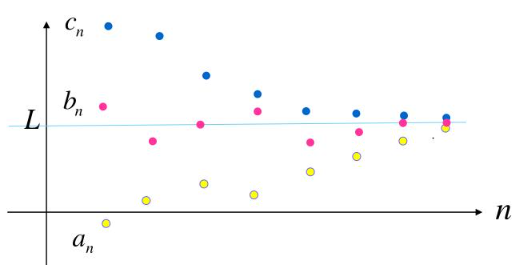
\includegraphics[width=0.7\linewidth]{squeeze.png}
    \end{figure}
\end{frame}

\begin{frame}{例}
    求
    \[
    \lim_{n\rightarrow\infty}\left(\frac{1}{n^2+n+1}+\frac{2}{n^2+n+2}+\cdots+\frac{n}{n^2+n+n}\right)
    \]
\end{frame}

% -------------------------------------------------------
% \section*{}
% \begin{frame}
% \vspace{25pt}
% \[
% \text{\Huge Office Hour}
% \]
% \end{frame}

\end{document}